\documentclass[11pt]{article}

\usepackage[margin=0.75in]{geometry}
\usepackage{url}
\usepackage{graphicx}
\usepackage{float}
\usepackage{amsmath}
\usepackage[utf8]{inputenc}
\PassOptionsToPackage{usenames,dvipsnames,svgnames}{xcolor}
\usepackage{tikz}
\usetikzlibrary{arrows,positioning,automata}
\graphicspath{ {../../graphs/} }
\usepackage{hyperref}
\usepackage{url}
\usepackage{listings}

%%% Date formatting to include month and year only
\usepackage{datetime}
\newdateformat{monthyeardate}{\monthname[\THEMONTH] \THEYEAR}

%%% Title
\title{A reproducible re-analysis of the RNA-seq study of
  \href{http://www.nature.com/neuro/journal/v18/n1/abs/nn.3898.html}{Jaffe
  \textit{et al.} (2014)}
}
%\subtitle{Reproducible Research in Bioninformatics and Statistics}

\author{ Nima Hejazi \\
  \href{mailto:nh@nimahejazi.org}{\texttt{nh@nimahejazi.org}}
}
\date{\monthyeardate\today}
\bibliographystyle{siam}

%%% Begin document
\begin{document}
\maketitle


\section{Introduction}
The present project concerns the re-analysis of transcriptomic data from the
study described in the paper
\href{http://www.nature.com/neuro/journal/v18/n1/abs/nn.3898.html}
{``Developmental regulation of human cortex transcription and its clinical
relevance at base resolution''}, Jaffe \textit{et al.}, \textit{Nature
Neuroscience}. This document details the full bioinformatical and statistical
pipeline used to pre-process and analyze data from the aforementioned study.
\textit{As the full codebase produced for this re-analysis cannot be adequately
contained in a single document, please consult the GitHub repository for this
project at \url{https://github.com/nhejazi/neurodevstat} to examine all scripts
in detail.}


\section{Pseudo-alignment of RNA-seq reads}
In order to quantify RNA-Seq reads, alignment against a reference transcriptome
must be performed. Here, we take advantage of \textbf{pseudo-alignment} to
probabilistically align reads using the \textbf{Kallisto} software pacakge.
Below, we describe pseudo-alignment and the results of its application to the
Jaffe \textit{et al.} data. Pseudo-alignment of reads constituted the primary
pre-processing step necessary for re-analysis of the data; for all scripts in
the pre-processing pipeline, see this GitHub link:
\url{https://github.com/nhejazi/neurodevstat/tree/master/preprocess}.


\subsection{Summary of pseudo-alignment procedure}
Pseudo-alignment is a novel process for quantifying a set of samples of RNA-Seq
reads by performing partial matching against a reference transcriptome. The
novel pseudo-alignment process, implemented in the command line tool
\textbf{kallisto}, takes into account all of the information contained in a set
of reads while reducing the computational burden imposed by more traditional
alignment techniques. For a complete description of pseudo-alignment, consult
the paper {\href{http://www.nature.com/nbt/journal/v34/n5/full/nbt.3519.html}
{``Near-optimal probabilistic RNA-seq quantification''}}, Bray \textit{et al.},
\textit{Nature Biotechnology}, 2016.


\subsection{Results of pseudo-alignment procedure}
Using a publicly
available trascriptome assembled from the \textbf{GRCh38} \textit{Homo sapiens}
genome, sets of paired-end RNA-Seq reads for each of the 12 subjects involved in
the study were pseudo-aligned, resulting in count tables mapping each set of
reads to \textbf{173,259} transcriptomic objects. \textit{Please note that while
similar quantification tools (e.g., Cufflinks) produce estimates of mappings of
isoforms, kallisto provides estimates of transcript abundance}. Tables of
pseudocounts are produced for each set of paired-end RNA-Seq reads for each
subject in a tab-separated file format; these files are suitable for
concatenation into a single count table containing quantification results for
all subjects, which, after summarizing transcripts at the gene level, can be
used as input for statistical analysis.


\subsection{Sample code for pseudo-alignment with Kallisto}
The Kallisto software package was used to perform pseudo-alignment of paired-end
RNA-seq reads. After installation, Kallisto is available as a command-line tool.
In order to invoke the Kallisto pseudo-aligner on each pair of RNA-seq reads, a
wrapper script was written (in Python) to iteratively pass calls to the shell
to invoke the pseudo-aligner. The wrapper script is available on GitHub at
\url{https://github.com/nhejazi/neurodevstat/blob/master/preprocess/04_pseudoAlign.py}.
\textbf{Excerpted code is displayed below:}

\begin{lstlisting}[language=Python]
  import os
  import sys
  import subprocess
  import numpy as np

  dir_data = os.path.abspath(os.getcwd() + "/data/" + str(data_dir))
  dir_fastq = dir_data + "/" + fastq_dir
  dir_out = dir_data + "/" + out_dir

  samples = [s[:10] for s in os.listdir(dir_fastq)]
  samples = list(np.unique(samples))

  for i in samples:
      pseudoalign = ("kallisto quant -i" + " " +
                     "./data/Homo_sapiens.GRCh38.rel79.idx -o" + " " +
                     str(dir_data) + "/" + str(out_dir) + "/" + str(i) + " " +
                     "-b 100" + " " + dir_fastq + "/" + str(i) + "_1.fastq.gz"
                     + " " + dir_fastq + "/" + str(i) + "_2.fastq.gz")
      subprocess.call(pseudoalign, shell = True)
\end{lstlisting}


\section{Gene-level summarization of transcripts}
To prepare for statistical analysis, the R package \textbf{tximport} was used
to summarize the transcripts quantified by the \textbf{Kallisto} pseudo-aligner
at the level of known genes. This step in the pre-processing pipeline is
necessary in order to justify the downstream use of popular software packages
for statistical modeling. R scripts for performing this stage of
bioinformatical and statistical pre-processing are available in the
\textit{munge} subdirectory of the GitHub repository for this project (see this
link \url{https://github.com/nhejazi/neurodevstat/tree/master/munge}).
\textbf{Excerpted code for gene-level summarization is displayed below:}

\begin{lstlisting}[language=R]
  # summarize data from transcript to genes for modeling and inference
  txdf <- transcripts(EnsDb.Hsapiens.v79, columns = c("tx_id", "gene_name"),
                      return.type = "DataFrame")
  tx2gene <- as.data.frame(txdf)
  txi <- tximport(filenames, type = "kallisto", tx2gene = tx2gene,
                  reader = read_tsv) #, countsFromAbundance = "scaledTPM")

  pseudocounts_genes <- as.data.frame(txi$counts)
  colnames(pseudocounts_genes) <- sapply(strsplit(filenames, split = "/"),
                                         function(x) x[9])
  pseudocounts_genes$geneID <- rownames(pseudocounts_genes)
\end{lstlisting}


\section{Statistical analysis at the level of genes}

\subsection{Pre-processing of (pseudo)counts with Limma "voom"}
In order to analyze differential expression after summarizing transcripts at the
gene level, the linear modeling method of the popular R package \textbf{Limma}
was employed, including the "voom" transformation for analyzing RNA-seq digital
sequencing data in the form of counts (or, in this case pseudocounts). In order
to adequately use this transformation, we first filter out all genes for which
there were less than 10 mapped reads across subjects \textit{on average}. After
this filtering step, the "voom" transformation, including quality weights for
samples, was performed. Sample code and the resultant plot are displayed below:

\begin{lstlisting}[language=R]
  v_simple <- voomWithQualityWeights(pseudocounts_filtered, design_simple,
                                     normalization = "scale", plot = TRUE)
\end{lstlisting}

\begin{figure}[H]
\centering
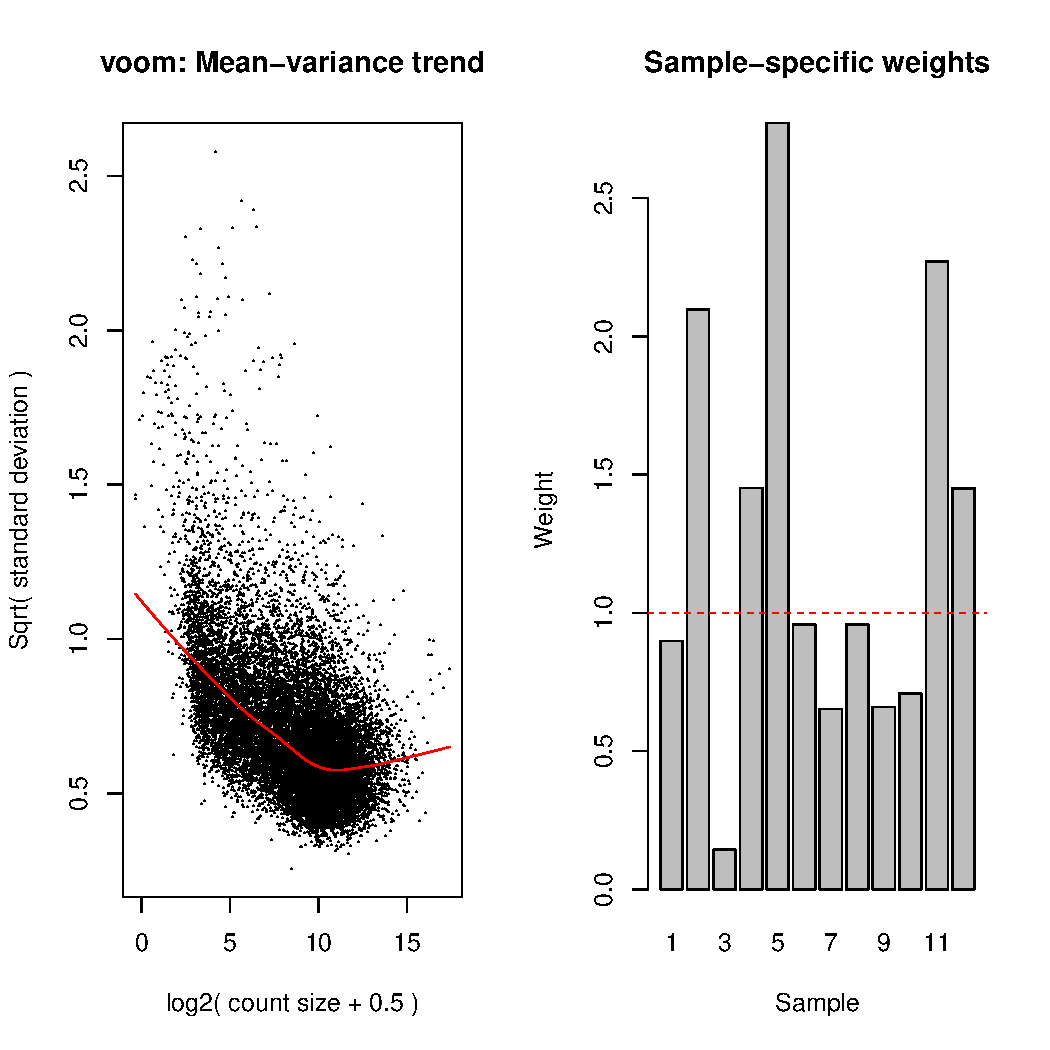
\includegraphics[scale=0.8]{voomTrend_simplemod.pdf}
\caption{Linear mean-variance trend and sample-specific weighting.}
\end{figure}


\subsection{Statistical analysis via linear modeling with Limma}
After summarizing transcripts at the gene level and generating subject-specific
weights via the "voom" transformation, the standard linear modeling method of
\textbf{Limma} was employed to analyze differential expression. Using a simple
design matrix, including terms only for an intercept and sample status (adult
vs. fetal), linear models were fit to each gene, and a moderated t-statistic is
computed based on the difference of means and a shrunken variance estimate, the
latter computed from performing empirical Bayes shrinkage across all genes. The
resulting table of differential expression is cleaned using the \textbf{dplyr}
R package, with the table being used downstream for data visualization. For
scripts used in the statistical analysis, see the \textit{src} subdirectory in
the project repo:
\url{https://github.com/nhejazi/neurodevstat/tree/master/src}. \textbf{Sample
code for linear modeling with Limma is given below:}

\begin{lstlisting}[language=R]
  vfit_simple <- limma::lmFit(v_simple)
  vfit_simple <- limma::eBayes(vfit_simple)
  tt1 <- limma::topTable(vfit_simple,
                         coef = which(colnames(design_simple) == "type"),
                         adjust.method = "BH", number = Inf,
                         sort.by = "none", confint = TRUE)

  # clean up topTable output to generate results tables
  tt_out1 <- tt1 %>%
    dplyr::mutate(
      geneID = geneIDs,
      lowerCI = exp(CI.L),
      FoldChange = exp(logFC),
      upperCI = exp(CI.R),
      pvalue = I(P.Value),
      fdrBH = I(adj.P.Val)
    ) %>%
    dplyr::select(which(colnames(.) %ni% colnames(tt1)))
\end{lstlisting}


\subsection{Data Visualization and Results}
After assessing differential expression via the suite of statistical tests
available in the linear modeling R package \textbf{Limma}, genes were ranked
by the computed Benjamini-Hochberg FDR and a volcano plot (using
\textbf{ggplot2}) of the results was generated, with labels for the \textit{the
top 25 genes}. Just as in the case of statistical analyses performed, all code
for data visualization can be found in  the \textit{src} subdirectory of the
project GitHub repository (available at this link
\url{https://github.com/nhejazi/neurodevstat/tree/master/src}). \textbf{Sample
code for and the resultant volcano plot are given below:}

\begin{lstlisting}[language=R]
  p3 <- ggplot(tt_out1_gg, aes(x = logFC, y = logPval)) +
    geom_point(aes(colour = color)) +
    geom_text(aes(label = ifelse(top != 0, as.character(geneID), '')),
              hjust = 0, vjust = 0, check_overlap = TRUE) +
    xlab("log2(Fold Change)") + ylab("-log10(raw p-value)") +
    ggtitle("Volcano Plot \n (from simple model)") +
    scale_colour_manual(values = pal2[1:3], guide = FALSE)
  print(p3)
\end{lstlisting}

\begin{figure}[H]
\centering
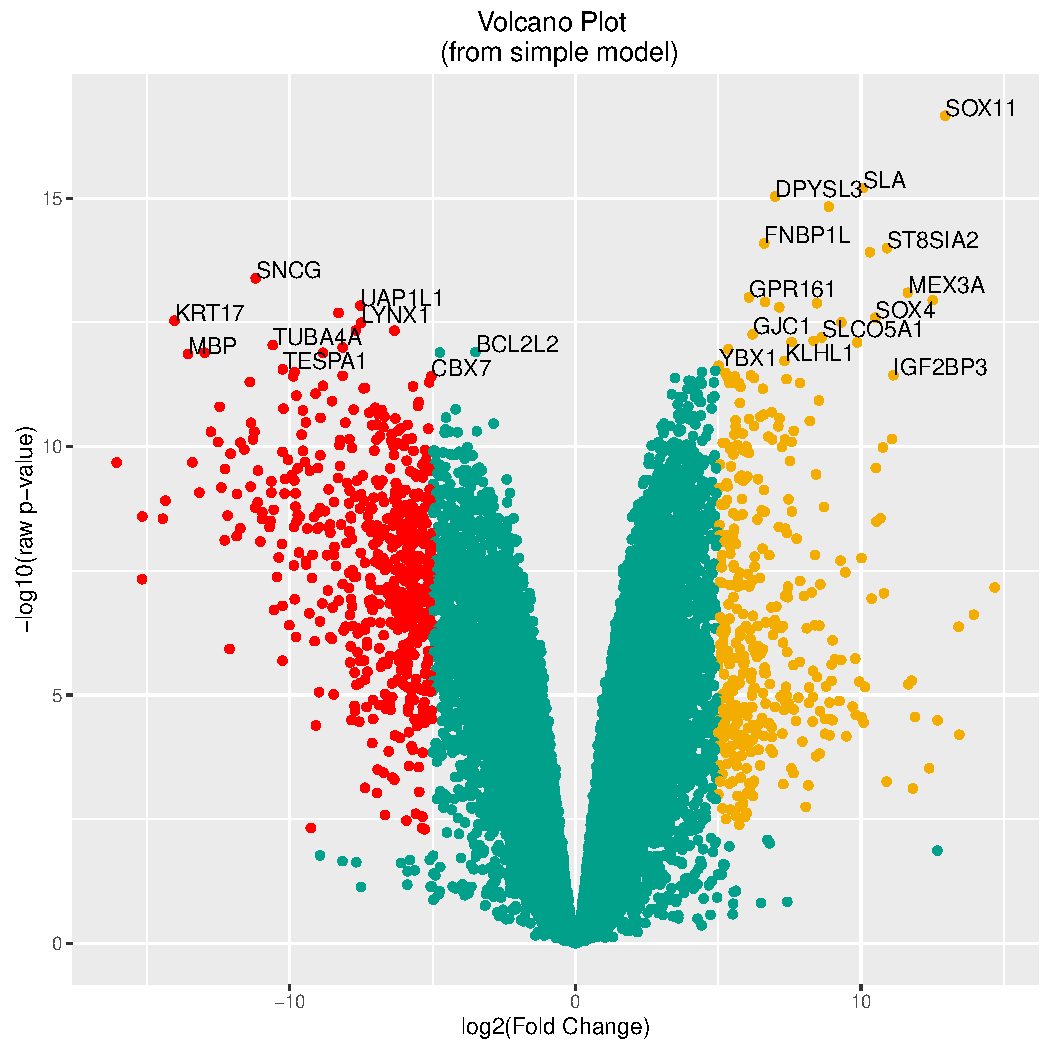
\includegraphics[scale=0.8]{volcano_simplemod_genes.pdf}
\caption{Volcano plot of \textbf{Limma} results using \textbf{ggplot2}.}
\end{figure}


\section{Reproducibility notice}
In the spirit of computationally reproducible research, the material used
producing all of the analyses reported on in this project is publicly available
on GitHub at \url{https://github.com/nhejazi/neurodevstat}. Minimally sufficient
documentation is provided so that all reported results can be reproduced with
relative ease. With any concerns, contact the author at
\href{mailto:nh@nimahejazi.org}{nh@nimahejazi.org}. \textit{A table of the core
software packages and the versions used for this analysis is given below:}

\begin{center}
\begin{tabular}{ |c|c| }
  \hline
  \textit{\textbf{Software}} & \textit{\textbf{Version}} \\
  \hline
  R (language) & 3.3.2 \\
  \hline
  Python (language) & 3.5.2 \\
  \hline
  Kallisto (pseudoalignment tool) & 0.42.5 \\
  \hline
  EnsDb.Hsapiens.v79 (R package) & 1.1.0 \\
  \hline
  tximport (R package) & 1.2.0 \\
  \hline
  limma (R package) & 3.30.0 \\
  \hline
  ggplot2 (R package) & 2.1.0 \\
  \hline
  dplyr (R package) & 0.5.0 \\
  \hline
\end{tabular}
\end{center}


\end{document}
